% Options for packages loaded elsewhere
\PassOptionsToPackage{unicode}{hyperref}
\PassOptionsToPackage{hyphens}{url}
%
\documentclass[
  12 pt,
  a4paper,
]{article}
\usepackage{amsmath,amssymb}
\usepackage{setspace}
\usepackage{iftex}
\ifPDFTeX
  \usepackage[T1]{fontenc}
  \usepackage[utf8]{inputenc}
  \usepackage{textcomp} % provide euro and other symbols
\else % if luatex or xetex
  \usepackage{unicode-math} % this also loads fontspec
  \defaultfontfeatures{Scale=MatchLowercase}
  \defaultfontfeatures[\rmfamily]{Ligatures=TeX,Scale=1}
\fi
\usepackage{lmodern}
\ifPDFTeX\else
  % xetex/luatex font selection
  \setmainfont[]{Times New Roman}
\fi
% Use upquote if available, for straight quotes in verbatim environments
\IfFileExists{upquote.sty}{\usepackage{upquote}}{}
\IfFileExists{microtype.sty}{% use microtype if available
  \usepackage[]{microtype}
  \UseMicrotypeSet[protrusion]{basicmath} % disable protrusion for tt fonts
}{}
\makeatletter
\@ifundefined{KOMAClassName}{% if non-KOMA class
  \IfFileExists{parskip.sty}{%
    \usepackage{parskip}
  }{% else
    \setlength{\parindent}{0pt}
    \setlength{\parskip}{6pt plus 2pt minus 1pt}}
}{% if KOMA class
  \KOMAoptions{parskip=half}}
\makeatother
\usepackage{xcolor}
\usepackage[margin=1in]{geometry}
\usepackage{graphicx}
\makeatletter
\def\maxwidth{\ifdim\Gin@nat@width>\linewidth\linewidth\else\Gin@nat@width\fi}
\def\maxheight{\ifdim\Gin@nat@height>\textheight\textheight\else\Gin@nat@height\fi}
\makeatother
% Scale images if necessary, so that they will not overflow the page
% margins by default, and it is still possible to overwrite the defaults
% using explicit options in \includegraphics[width, height, ...]{}
\setkeys{Gin}{width=\maxwidth,height=\maxheight,keepaspectratio}
% Set default figure placement to htbp
\makeatletter
\def\fps@figure{htbp}
\makeatother
\setlength{\emergencystretch}{3em} % prevent overfull lines
\providecommand{\tightlist}{%
  \setlength{\itemsep}{0pt}\setlength{\parskip}{0pt}}
\setcounter{secnumdepth}{-\maxdimen} % remove section numbering
\ifLuaTeX
\usepackage[bidi=basic]{babel}
\else
\usepackage[bidi=default]{babel}
\fi
\babelprovide[main,import]{spanish}
\ifPDFTeX
\else
\babelfont{rm}[]{Times New Roman}
\fi
% get rid of language-specific shorthands (see #6817):
\let\LanguageShortHands\languageshorthands
\def\languageshorthands#1{}
\ifLuaTeX
  \usepackage{selnolig}  % disable illegal ligatures
\fi
\usepackage{bookmark}
\IfFileExists{xurl.sty}{\usepackage{xurl}}{} % add URL line breaks if available
\urlstyle{same}
\hypersetup{
  pdflang={es-ES},
  hidelinks,
  pdfcreator={LaTeX via pandoc}}

\title{U1 EXERCICIS. INTRODUCCIÓ ALS SISTEMES INFORMÀTICS}
\author{}
\date{\vspace{-2.5em}}

\begin{document}
\maketitle

{
\setcounter{tocdepth}{2}
\tableofcontents
}
\setstretch{1.5}
\newpage
\renewcommand\tablename{Tabla}

\subsection{1 Conversió de RGB}\label{conversiuxf3-de-rgb}

Els codis hexadecimals de colors RGB es representen amb 6 dígits: dos
per al component roig (Red), dos per al component verd (Green) i dos per
al component blau (Blue). Cada component és un número hexadecimal que
pots convertir a binari i també (SEPARANT de 2 en 2 a decimal).

\textbf{Instruccions per a cada cas:}

\begin{enumerate}
\def\labelenumi{\arabic{enumi}.}
\tightlist
\item
  Separar el codi hexadecimal en tres parts: una per al component
  vermell (R), una per al component verd (G) i una per al component blau
  (B).
\item
  Convertir cada part hexadecimal a decimal.
\item
  Convertir cada valor decimal a binari, assegurant-te que cada
  component binari sigui de 8 bits.
\end{enumerate}

Exemple de resolució per al cas \#FF5733:

\textbf{Hexadecimal:} \#FF5733\\
- R = FF\\
- G = 57\\
- B = 33

\textbf{Conversió a decimal:} - R = 16\emph{16\(^{1}\) + 15 = 255\\
- G = 5}16\(^{1}\) + 7 = 87\\
- B = 3*16\(^{16}\) + 3 = 51

\textbf{Conversió a binari (8 bits):} - R = 11111111\\
- G = 01010111\\
- B = 00110011

\textbf{Fes els següents exemples:}

\begin{enumerate}
\def\labelenumi{\arabic{enumi}.}
\tightlist
\item
  \textbf{\#4A90E2}\\
\item
  \textbf{\#7D3F8C}\\
\item
  \textbf{\#2ECC71}
\end{enumerate}

\subsection{2 Conversió de IPv4}\label{conversiuxf3-de-ipv4}

Una IP4 està composada de 4 bytes (4 * 8 = 32 bits). Però la representem
per comoditat en decimal

Vegem l'exemple de conversió: Per convertir una adreça IP en IPv4 a
binari i hexadecimal, segueix aquests passos:

\textbf{Conversió a binari:}

\begin{itemize}
\tightlist
\item
  Separar l'adreça IP en els seus quatre octets: 192, 168, 1, 10.
\item
  Convertir cada octet a binari:
\end{itemize}

Exemple: \textbf{192.168.1.10} \textbf{192} en binari:\\
Decimal: 192\\
Binari: 11000000

\textbf{168} en binari:\\
Decimal: 168\\
Binari: 10101000

\textbf{1} en binari:\\
Decimal: 1\\
Binari: 00000001

\textbf{10} en binari:\\
Decimal: 10\\
Binari: 00001010

Per tant, l'adreça IP en binari és:\\
\textbf{11000000.10101000.00000001.00001010}

Com passaries a hexadecimal el binari resultant?

\textbf{Fes la conversió a binari i decimal de les IPs:}

\begin{enumerate}
\def\labelenumi{\arabic{enumi}.}
\item
  \textbf{10.2.2.2}
\item
  \textbf{172.217.3.110}
\item
  \textbf{151.101.1.67}
\item
  \textbf{13.226.32.32}
\end{enumerate}

\subsection{3 Octal}\label{octal}

Representa en octal i decimal els caracters especials i les lletres
següents d' ASCII ( et deixe al costa el seu valor en decimal )

\begin{enumerate}
\def\labelenumi{\arabic{enumi}.}
\tightlist
\item
  \textbf{\textless{} 60}
\item
  \textbf{@ 64}
\item
  \textbf{A 65}
\item
  \textbf{a 97}
\end{enumerate}

\subsection{4 Investigació}\label{investigaciuxf3}

Investiga i documenta molt breument com són les adreces MAC, com estan
compostes, com es guarden, ús\ldots{}

\subsection{5 Problema real amb taula de
codis}\label{problema-real-amb-taula-de-codis}

Fent la FCT en un Ajuntament, un administratiu que està registrant dades
electorals de la comarca ens planteja un problema que té amb el fitxer
\href{altres/resultatsSafor.csv}{resultatsSafor.csv} (descarrega-te'l).

El problema és que, en obrir-lo amb Calc de LibreOffice o MS Excel, veu
que alguns caràcters no són correctes tal i com mostra la Figura 1
(vocals amb accent gràfic, per exemple)

\begin{figure}
\centering
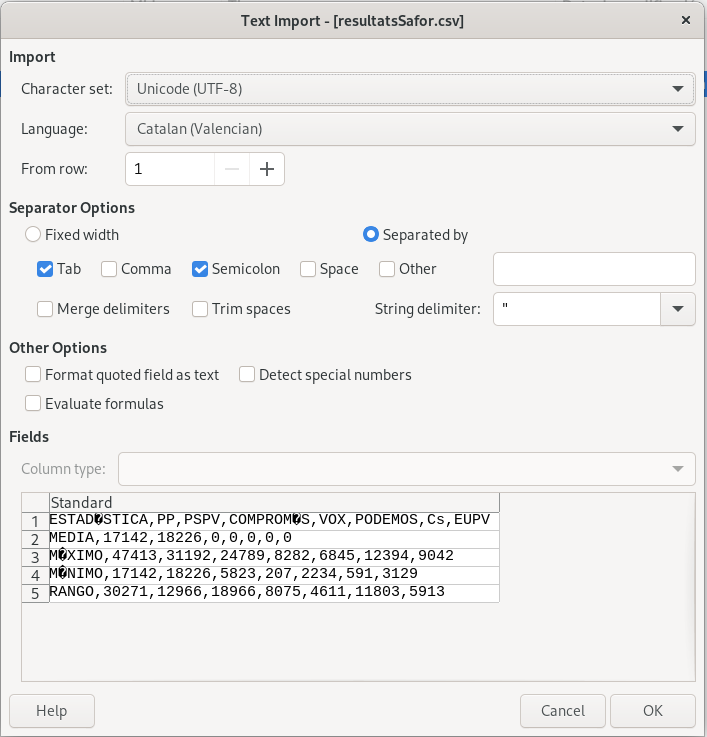
\includegraphics{png/resultatsSafor.png}
\caption{\emph{Figura 1: Importació de CSV}}
\end{figure}

A partir d'ací\ldots{}

\begin{enumerate}
\def\labelenumi{\arabic{enumi}.}
\tightlist
\item
  Raona i indica quin creus que és el problema.
\item
  Com ho solucionaries temporalment? 3 I de forma definitiva?
\item
  Creus que el fitxer prové d'una Base de Dades actualitzada?
\end{enumerate}

\end{document}
